\documentclass[letterpaper, 10 pt, conference]{ieeeconf}  % Comment this line out if you need a4paper

%\documentclass[a4paper, 10pt, conference]{ieeeconf}      % Use this line for a4 paper

\IEEEoverridecommandlockouts                              % This command is only needed if 
                                                          % you want to use the \thanks command

\overrideIEEEmargins                                      % Needed to meet printer requirements.

% See the \addtolength command later in the file to balance the column lengths
% on the last page of the document

% The following packages can be found on http:\\www.ctan.org
\usepackage{graphicx} % for pdf, bitmapped graphics files
\graphicspath{{../}}
\usepackage{epstopdf} % for postscript graphics files
\usepackage{mathptmx} % assumes new font selection scheme installed
\usepackage{times} % assumes new font selection scheme installed
\usepackage{amsmath} % assumes amsmath package installed
\usepackage{amssymb}  % assumes amsmath package installed
\usepackage[caption=false,font=footnotesize]{subfig}
\usepackage{fixltx2e}
\usepackage{float}

\title{\LARGE \bf
3D-PIV application for autonomous vehicles using monocular vision
}


\author{Eduardo Afonso$^{1}$ and Researcher$^{2}$% <-this % stops a space
\thanks{$^{1}$ Eduardo Afonso is coursing Control and Automation Engineering,
        Federal University of Lavras, Lavras - MG, Brazil.
        {\tt\small eduardo.afonso@engautomacao.ufla.br}}%
\thanks{$^{2}$ Researcheris with the Department of Electrical Engineering, Wright State University,
        Dayton, OH 45435, USA
        {\tt\small b.d.researcher@ieee.org}}%
}


\begin{document}


\maketitle
\thispagestyle{empty}
\pagestyle{empty}

\begin{abstract}


\end{abstract}
\section{INTRODUCTION}

Monocular vision comes being a flourishing field in autonomous vehicles. 
Several applications have presented solutions to current problems. 
Although in systems  of low computational cost remain a challenge. 


The Particle Image Velocimetry ($PIV$)\cite{Bastiaans} technique is used in many fields of 
knowledge, \cite{Story, Xu}, to calculate the velocity of fluids in different parts. 
Here, $PIV$ was adjusted for situation of autonomous vehicles, using a matching criteria based on 
the Pearson Correlation Coefficient ($PCC$)\cite{Miranda Neto} over the KITTI dataset\cite{Geiger}.





\section{THEORETICAL FUNDAMENT}

\subsection{THE PEARSON CORRELATION COEFFICIENT}

$PCC$ is used in statistical analyses, pattern recognition and computer vision. 
It can be used to comparing two images in an object recognition system. 
The following equation describes the $PCC$ method for two gray scale digital images\cite{Eugene},
represented by the matrices $A$ and $B$ with $M$ elements each one,
\begin{equation}
r = \frac{\sum \limits_{i}^{M} (a_i-\mu_a)(b_i-\mu_b)}{\sqrt{\sum \limits_{i}^{M} (a_i-\mu_a)^2} \sqrt{\sum\limits_{i}^{M} (b_i-\mu_b)^2}},
\end{equation}
\begin{equation}\label{eq:PCC}
 r=PCC(A,B)
\end{equation}

where $a_i$ is the intensity of the i-th pixel in the  matrix $A$, 
$b_i$ is the intensity of the i-th pixel in the matrix $B$, 
$\mu_a$ is the mean intensity of $A$,
$\mu_b$ is the mean intensity of $B$ and
$r$ is the correlation coefficient \cite{Miranda Neto}.


\subsection{PARTICLE IMAGE VELOCIMETRY}

$PIV$ is a technique to determine the  velocity field of objects from a stream of images\cite{Bastiaans}.
The result of the $PIV$ is given as a vector field, showing for each particle the direction, sense and intensity of velocity. 
Moreover, the $PIV$ can be calculated for different objects in the same image.
For this purpose, the $PIV$ technique divides the frame 1 in regions (particles), after frame 1 and 2 are correlated 
using comparative method, so a vector or a field of vector is generated that represent the displacement. Thus, we have 
displacement and time of computing, applying of conception of derivate it is possible to estimate relative velocity.

\begin{figure}[H]
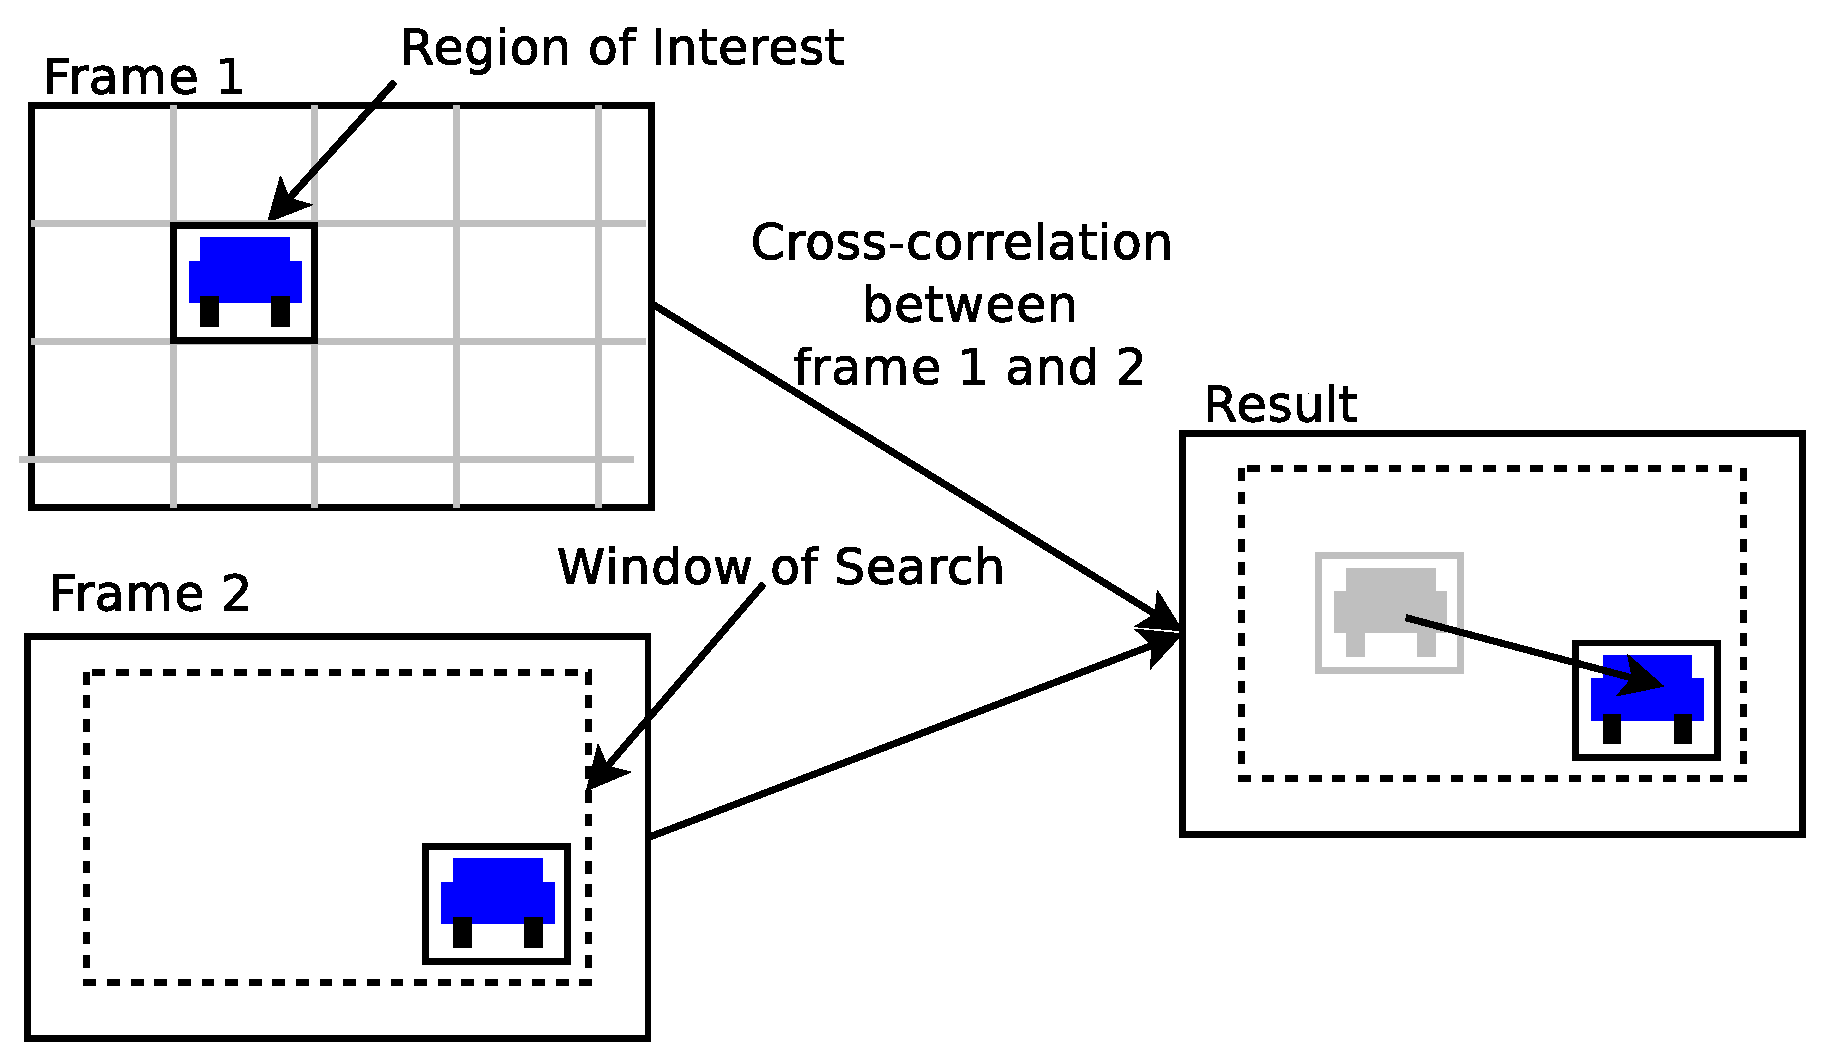
\includegraphics[width=\columnwidth]{images/explanationPIV.eps}
\caption{The PIV operation comparing two frames}
\label{fig:system}
\end{figure}

The figure above shows how PIV works and also demonstrates the relation between Region of Interest (ROI) and 
Window of Search (WOS). WOS involves ROI because WOS is considered the possibles regions that object could be. 
WOS don't need necessary fill whole image. If WOS is large, so we have an augment of computing but 
if WOS is small, object can be lost. In our application, we determine WOS from 1,5 of ROI. For example, 
if ROI is 200x300 so we have WOS of 300x450. It means object will be in anywhere in this WOS. This consideration can be
proven by testes in environment of low velocity of objects (velocity in cities and roads).

\begin{figure}[H]
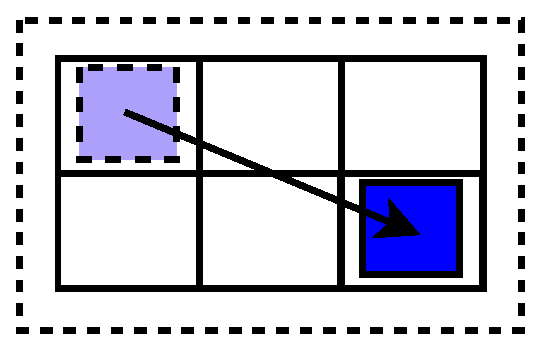
\includegraphics[width=\columnwidth]{images/WOSdivided.eps}
\caption{WOS is divided in windows of same dimensions of ROI}
\label{fig:system}
\end{figure}

ROI is one of most important part of PIV, because it contains followed object. An window of same dimension of ROI is displaced
along of whole WOS in frame 2, like showed in figure above. One comparison is done and assigned a value in each displacement. 
When process finishes, the more height value is considered the new place of ROI. It means that object displaced of initial 
position in frame 1 to found position in frame 2.


\section{SYSTEM DESCRIPTION}
The purpose of this algorithm is to make a (3D) tracking system, producing position informations 
about the followed target.
These informations will be relevant to define parameters 
as: the relative velocity, the factor of approaching and of departure.

The proposed algorithm is shown in the Fig. \ref{fig:system};
this begin with a key frame image where a initial Region Of Interest ($ROI$) is determined; 
the system then receive a stream of image frames and the tracking system 
enters in looping to follow the target in the next frames.
In this case, to difference of $PIV$, the compared images are 
the current image in the image stream and the current $ROI$.

\begin{figure}[bhp]
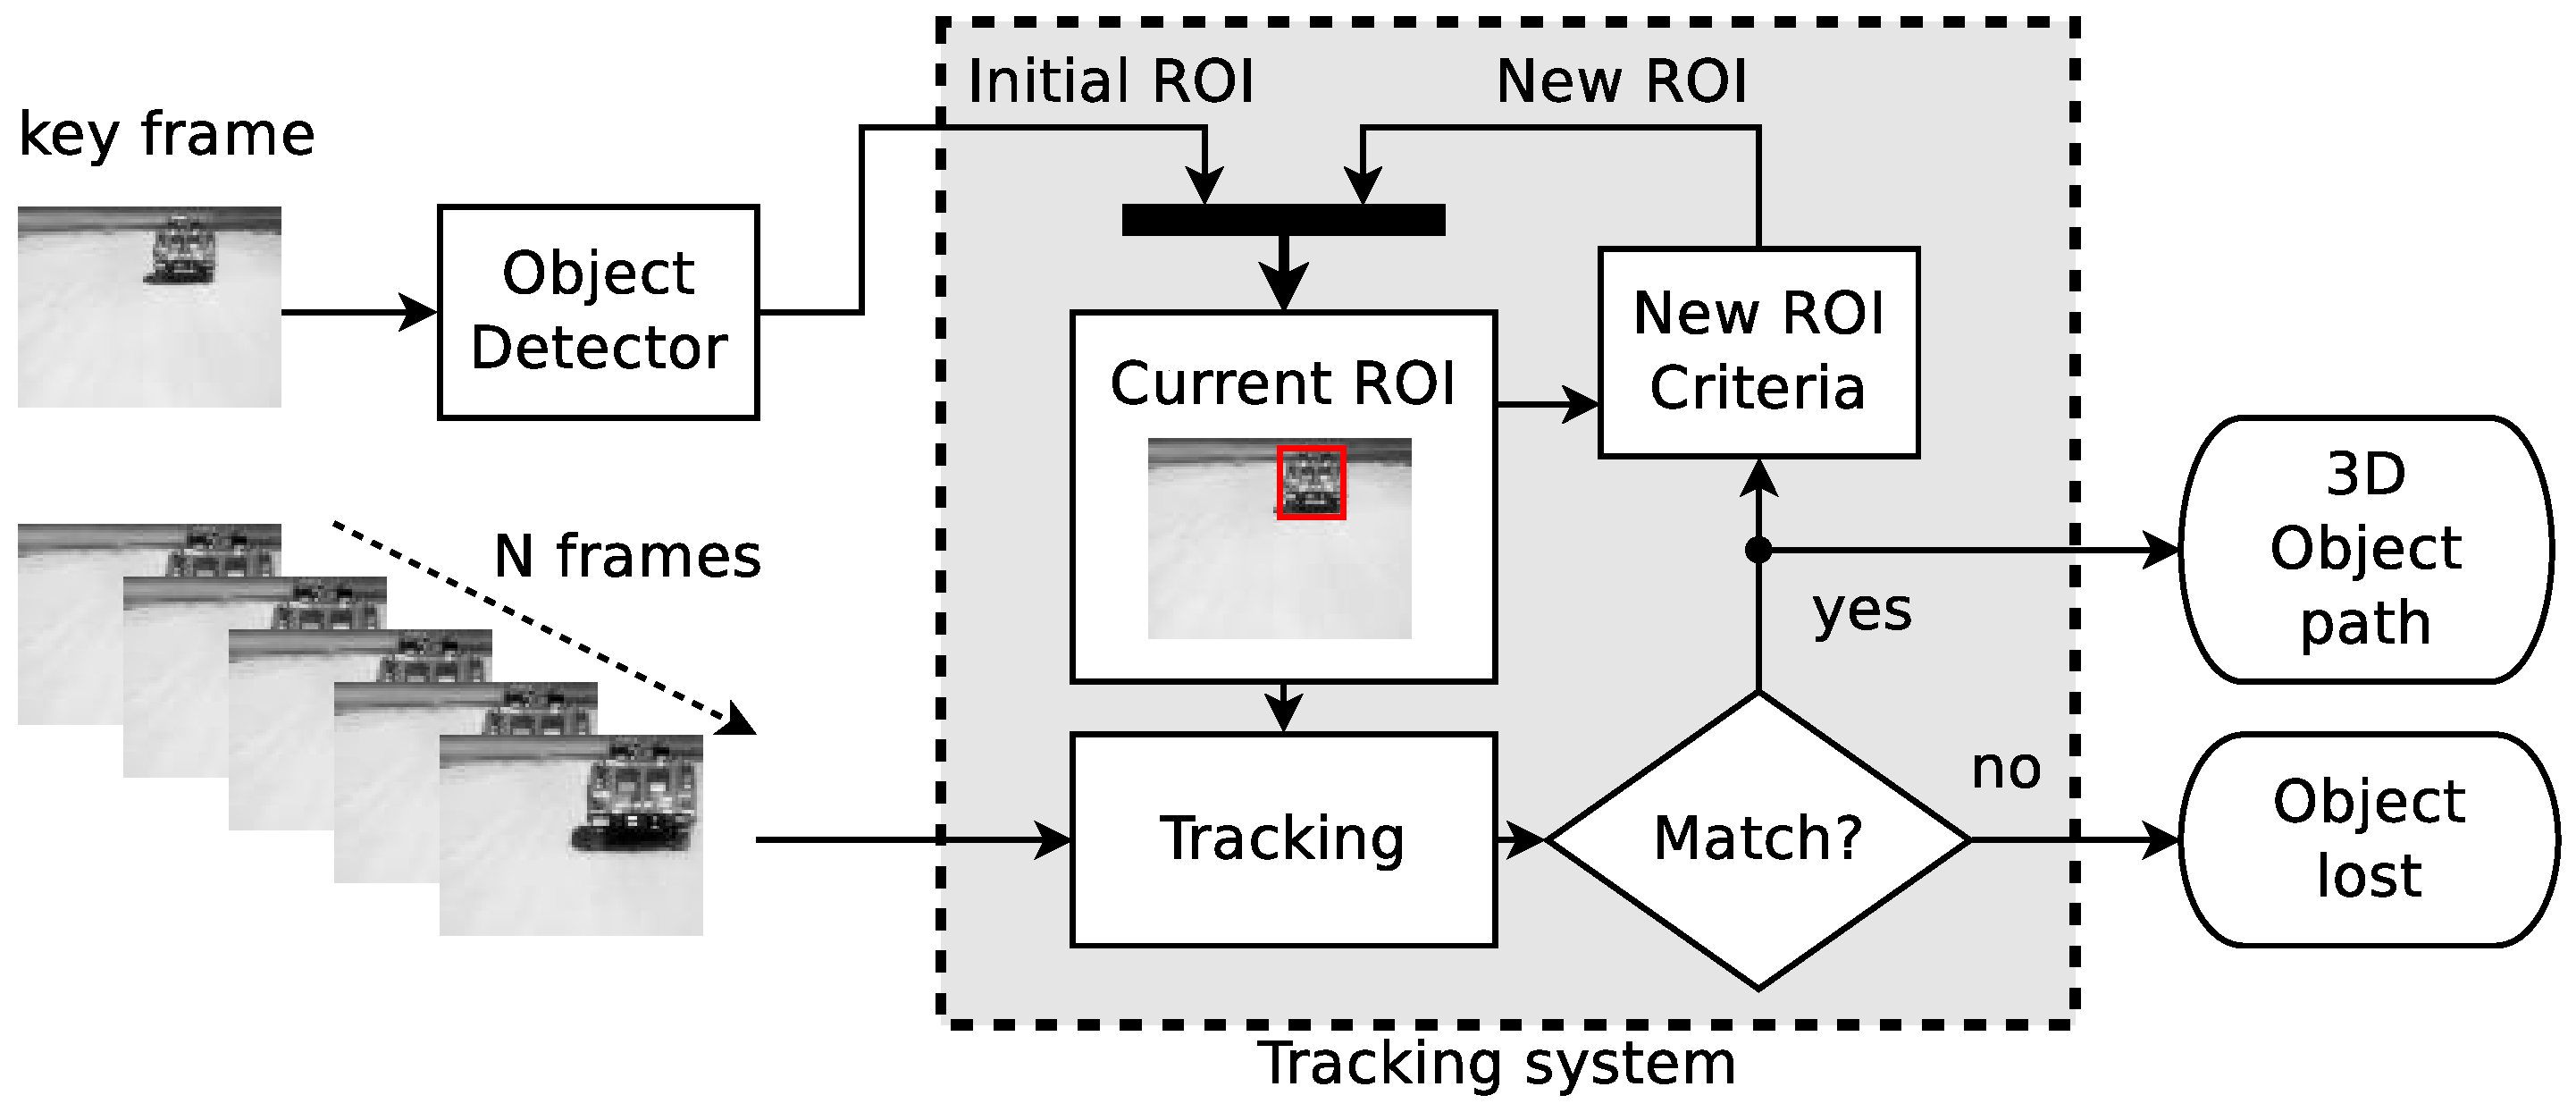
\includegraphics[width=\columnwidth]{images/figure1-diagram1.eps}
\caption{With the current $ROI$ selected, a highest value of $PCC$, between the $ROI$ 
and the Window Of Search ($WOS$) of current frame, identifies the target; 
the result of search is a displacement vector
between the first and last position of object. 
After, this processing is made again to the next frames.}
\label{fig:system}
\end{figure}

In a 2 dimensional analysis, the tracked objects given us information about your horizontal 
and vertical position, and your relative perpendicular velocity respect to the observer.
When the target is analyzed in 3 dimensions, 
the initial $ROI$ has the position $(x=x_0,y=x_0,d=d_0=1)$;
where, $x_0$ and $y_0$ represent a position (horizontal and vertical) in the analyzed image,
and $d_0=1$ represents the initial depth position of object in the $ROI$ (normalized by definition to $1.0$).
Thus, all the results of depth will be relatives to this value, 
In this sense only can be calculated, relative values of
velocity and the factor of approaching or departure. 

%Diagrama1
 %A gente vai explicar o algoritmo como uma caixa fechada , que coisa entra e que coisa sai
 %e os parametros a sintonizar.
 % como usar ele quando implementado, como se fosse uma caixa preta.


\section{ALGORITHM DESCRIPTION}
 
%DiagramaX

\subsection{MULTI-SCALE MATCH CRITERIA}
The match criteria to track object at images is based in the $PIV$ technique; 
where, a ROI and a Window Of Search ($WOS$) is defined; and is 
verified the similarity of $ROI$ over any part of $WOS$ using $PCC$. 
So that, the highest coefficient of Pearson determines the new location of the object.

Figure \ref{fig:multires}(a) shows a application in 2 dimensions, where
the $ROI$ information is searched, in the same scale,  in the entire image.

The Figure \ref{fig:multires}(b) reveals how the dimension of depth was included and
the search is made in different scales (layers); so that, in 3 dimensions the target 
also is found through the highest $PCC$ among $WOS$, but the object found may be 
bigger or smaller, depending of in which layer the match happens. 
In both cases, before of be compared, the analyzed region in the $WOS$ was 
rescaled to have the same size that the $ROI$.

\begin{figure}[H]
\centering
  \subfloat[]{\label{subfig:(a)} 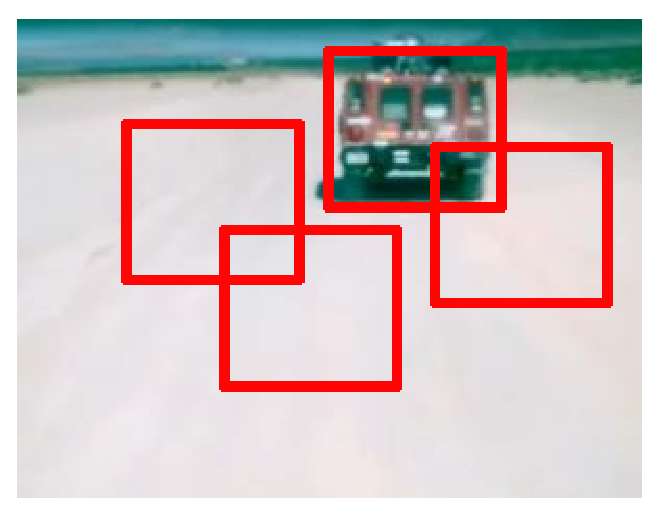
\includegraphics[width=.5\columnwidth]{images/figure2a.eps}}
  \subfloat[]{\label{subfig:(b)} 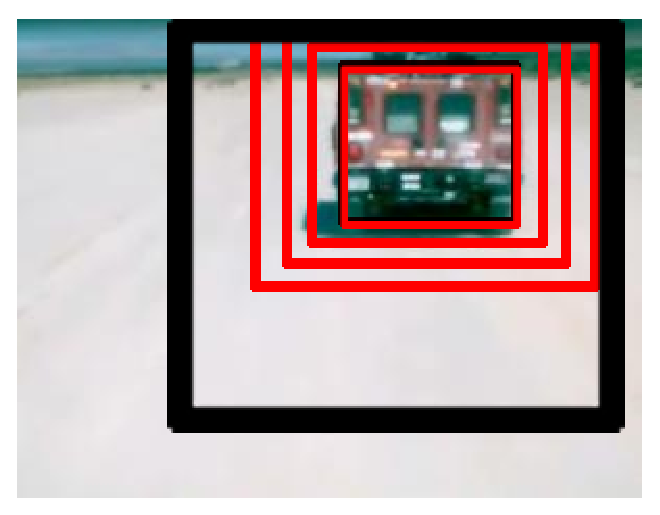
\includegraphics[width=.5\columnwidth]{images/figure2b.eps}}
  \caption{The red boxes show the analyzed regions and the black boxes represent the $WOS$. 
  (a) The regions are compared in the same scale with the $ROI$. 
  (b) The red boxes are used to different layers in different scales.}
  \label{fig:multires}
\end{figure}




%onde estava, onde esta agora
%que tamanho tinha que tamanho tem.
\subsubsection{MULTI-LAYER 3D APPROXIMATION}
The multi-layer is a technique to track objects that move in 3 dimensions. The layers are organized of the smallest to the biggest, 
there is a rate which layers increase. With this proceeding, the algorithm is capable of track objects that in second scene was larger than first.\\

%usa Multi-resolution match criteria e explica isso dos tamanhos

\subsubsection{FACTOR OF APPROACHING - RELATIVE VELOCITY}
Factor of approaching is a dimensionless number related to the rate of approaching or departure of an object to the camera. The factor
is determined how showed at equation 2:

\begin{equation}
\centering
\everymath{\displaystyle}
f_a = \frac{Area_r}{Area_f} 
\end{equation}

Where $f_a$ is the factor of approaching, $Area_r$ is area of ROI and $Area_f$ is area of current frame.\\
The factor has two means, e.g., if the rate of approaching increase quickly, so the target is approaching. Or the apposite, if factor decreases, thus 
object is departing.\\
Relative velocity is calculate using a simples equation of kinematic in physics:


\begin{equation}
\centering
\everymath{\displaystyle}
 v = \frac{\Delta s}{\Delta t}
\end{equation}

Where $v$ is relative velocity, $\Delta s$ is difference in between two pixels and $\Delta t$ is time of proceeding.\\
Velocity calculated is relative for simple reason that it is impossible to know the real distance between the camera and object in this
condition.\\

\subsection{RENEW ROI CRITERION}
%Diagrama2
The $ROI$ is an important element in the algorithm, therefore it will be used
as pattern to find a match of tracked target at the current image. 
The  question in this case is to know the best moment to refresh the $ROI$
with a new perspective of target. 
Here, we establish the criterion that; when the comparison of images return 
a $PCC$ value lower than $0.925$ and greater than $0.8$, then the $ROI$ is changed with the current 
analyzed region and a new position of $ROI$ is with $(x_i,y_i,d_i)$. 
Thus, it was adopted as $0.8$ the lower limit to a match case\cite{Eugene},
see Fig. \ref{fig:newroicri}. Values less than $0.8$ cause a  lost target alert.
Finally, it is important to note that if the $ROI$ is changed, the new $ROI$ is 
the real size of the analyzed region and not with the rescaled version used
in the calculus of the $PCC$.


\begin{figure}[H]
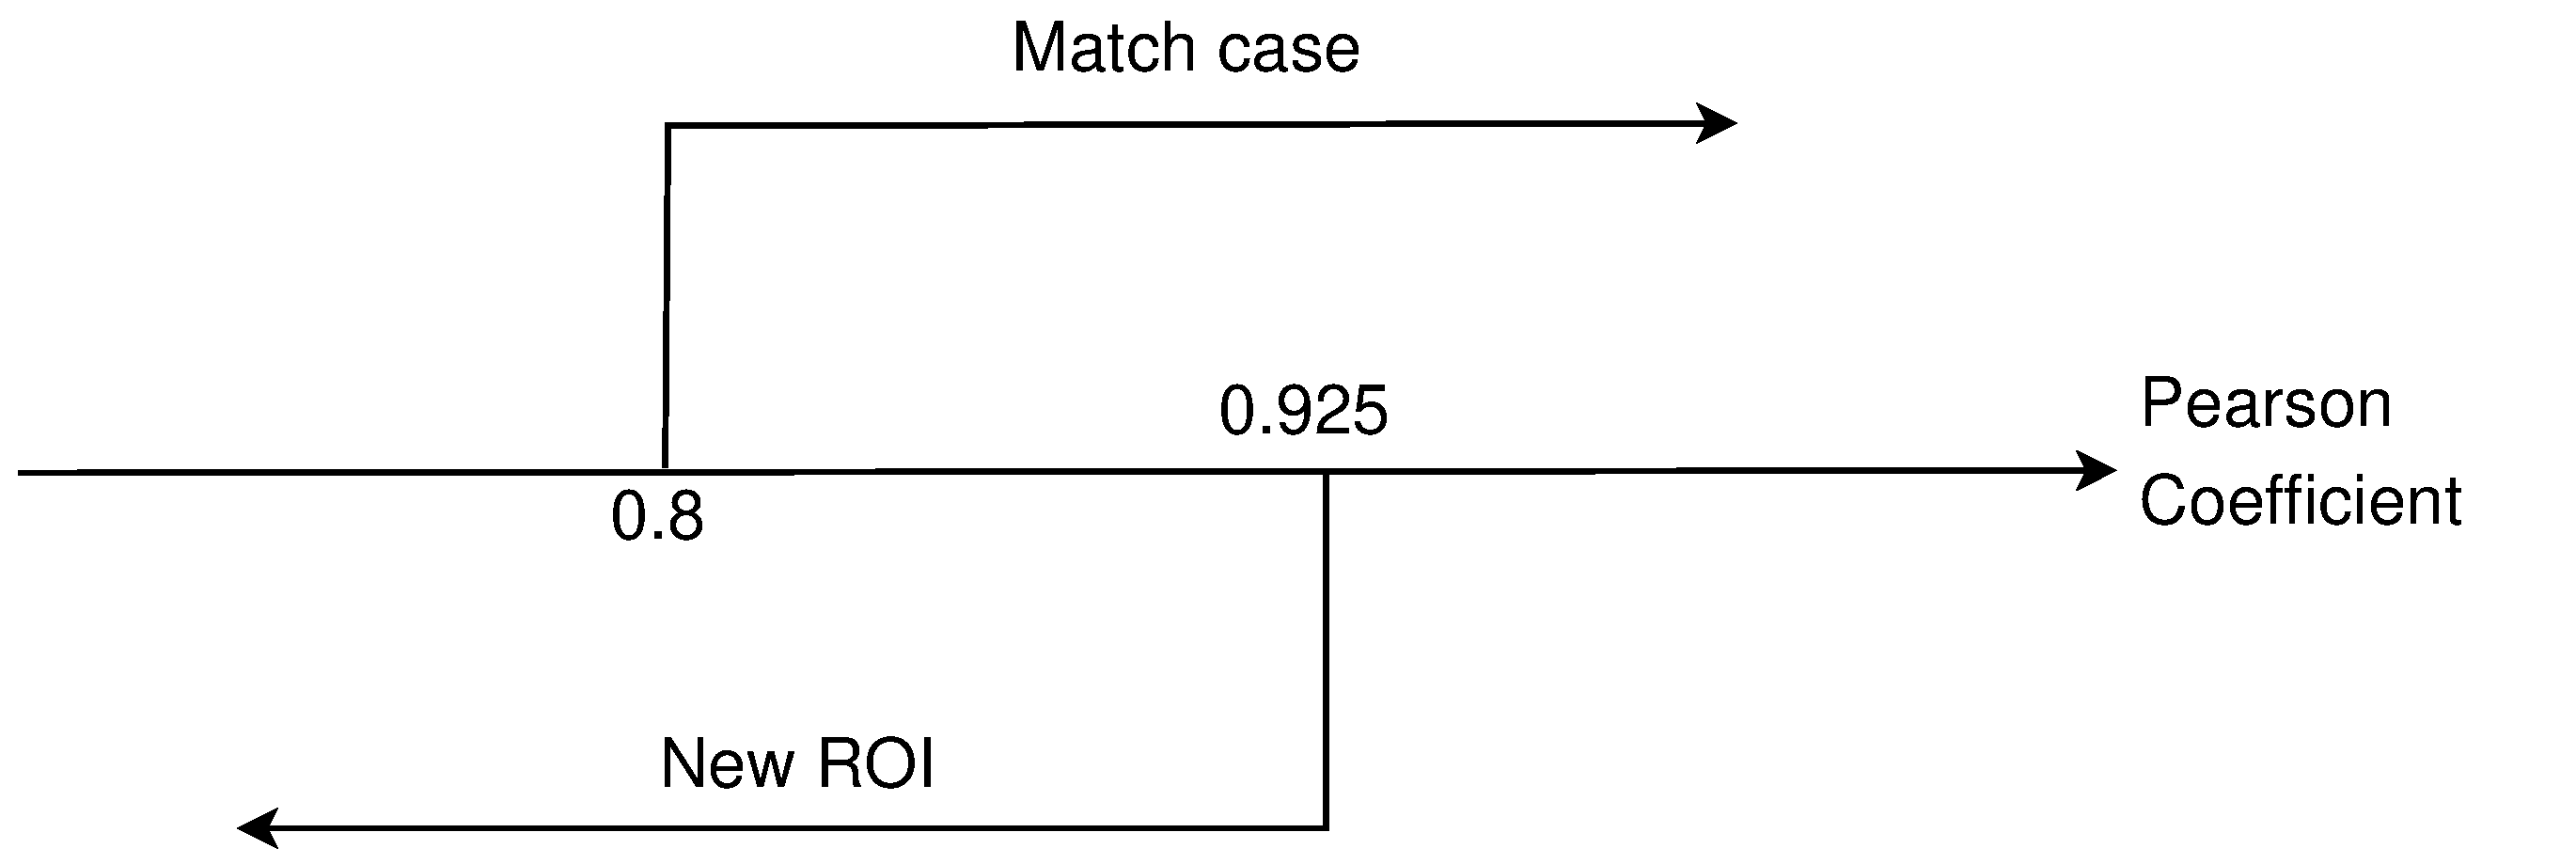
\includegraphics[width=\columnwidth]{images/figure3.eps}
\caption{When the comparison is greater than $0.8$, including numbers bigger than 
$0.925$, it means that the target was matched. But if two regions are compared 
and the $PCC$ is less than $0.925$ and greater than $0.8$, 
then the $ROI$ changes to the current analyzed region.}
\label{fig:newroicri}
\end{figure}

The Algorithm \ref{alg:newroi} shows the criteria described in the
Fig. \ref{fig:newroicri}; the $renew\_roi\_criteria()$ function, explained here,
it is used by the Algorithm \ref{alg:system} of Fig. \ref{fig:system}.

\begin{algorithm}[H]
 \KwData{Initial $ROI$, your position $P_0$, the current matched analysis region ($AR$), your position $P$ and the correlation $r$ between them. }
 \KwResult{The new $ROI$, your position and a status variable, $Found$. }

    $NEWP_0 \leftarrow  P_0$ \;
    $NEWROI \leftarrow  ROI$ \;
    
    \eIf{$0.8 \leq r$}
    {
      $Found \leftarrow True$\;
        message ``target found''\;
        \eIf{$r \leq 0.925$}
        {
            $NEWROI \leftarrow  AR$\;
            $NEWP_0 \leftarrow  P$\;
        }
    }
    {
      message ``target lost''\;
      $Found \leftarrow False$\;
    }
\Return  $\{NEWROI,~NEWP_0,~FOUND\}$\;
\label{alg:newroi}
\caption{$renew\_roi\_criteria(ROI,P_0,AR,P,r)$ function.}
\end{algorithm}
%The system needs to have a high level of reliability, so that the lower limit adopted 
%contributes to an operation with minimum of mistakes.


% descrio do sistemA
\section{NUMERICAL RESULTS}
%testes com diferentes parametros
% tabelas e graficos

\section{CONCLUSIONS}
From the presented examples,
it is possible to see that one application that uses the tracking
and the departure factor is related with risk of collision.
It is possible to estimate how of fast an object is departing,
and thus, if the  departure factor tends to zero or 
if the velocity of departure factor changes to lower negatives values every time, 
probably, there is a high risk of collision.

The $PIV$ technique has presented satisfactory results. 
Different kinds of information can be concluded, 
like: estimate collision using velocity of departure factor, 
tracking of objects in 2 or 3 dimensions and departure distance
relative to the first position of $ROI$. 
The simulations in both cases has given promissory results.

\addtolength{\textheight}{-12cm}

\section*{ACKNOWLEDGMENT}

%FAPEMIG\\
%numero de bolsa\\
%numero de projeto\\
%numero de aluno


\begin{thebibliography}{99}

\bibitem{Auoude} G.S. Auoude et al. Sampling-Based Threat Assessment Algorithms for Intersection Collisions Involving 
        Errant Drivers. IFAC Symposium on Intelligent Autonomous Vehicles, 2010.
        
	\bibitem{Bastiaans} R. J. M. Bastiaans, Cross-correlation PIV; theory, implementation and accuracy. 
        Eindhoven: Technische Universiteit Eindhoven, 2000. - EUT Report 99-W-OOl. - ISBN: 90-386-2851-X.
        
        \bibitem{Eugene} Y. K. Eugene and R.G. Johnston, The Ineffectiveness of the Correlation Coefficient for Image Comparisons.
        Technical Report LA-UR-96-2474, Los Alamos, 1996.
        
        \bibitem{Geiger} A. Geiger et al,
        Vision meets Robotics: The KITTI Dataset. International Journal of Robotics Research (IJRR), 2013.
        
        \bibitem{Jonas} T. Jonas, Real-Time Probabilistic Collision Avoidance for Autonomous Vehicles, Using Order Reductive 
        Conflict Metrics. Submitted to the Department of Aeronautics and Astronautics
	in partial fulfillment of the requirements for the degree of Doctor of Philosophy. Massachusetts Institute of Technology. June, 2003.
        
        \bibitem{Miranda Neto} A. Miranda Neto et al, Image Processing Using Pearson's Correlation Coefficient: 
        Applications on Autonomous Robotics. 
        Autonomous Robot Systems (Robotica), 2013 13th International Conference on, 2013.
	
	\bibitem{Story} A. Story et al, PIV measurements of the velocity field of a Newtonian Fluid in a stirred tank equipped 
	with the PMT type impeller.Technical Transactions - Chemistry. 2-Ch/2014.
	
	\bibitem{Woerner} K. Woerner, COLREGS-Compliant Autonomous Collision Avoidance Using Multi-Objective Optimization
	with Interval Programming. Submitted to the Department of Mechanical Engineering in partial fulfillment of the requirements for the 
	degrees of Naval Engineer and Master of Science in Mechanical Engineering. Massachusetts Institute of Technology. June, 2014.
	
	\bibitem{Xu} L. Xu, Computational fluid dynamics analysis and PIV validation of a bionic vortex flow 
	pulsatile LVAD.Technology and Health Care 23 (2015) S443?S451. DOI 10.3233/THC-150981. IOS Press, 2015.


\end{thebibliography}

\end{document}
